\begin{frame}{ROS Package}
    Used to gather the image and depth data from the Depth Camera Node, which publishes:
    \begin{itemize}
        \item Color image on ``\texttt{/depth\textunderscore camera/image\textunderscore raw}''
        \item Greyscale depth image on ``\texttt{/depth\textunderscore camera/depth/image\textunderscore raw}''
        \item PointCloud on ``\texttt{/depth\textunderscore camera/points}''
    \end{itemize}
    And store such data in files in the Common Workspace.
\end{frame}
\begin{frame}{Python Application - Bootstrapper}
    \begin{columns}
        \begin{column}{.25\linewidth}
            The bootstrapper launches three scripts:
            \begin{enumerate}
                \item Contour detector
                \item Pixel to World coordinates Converter
                \item Duplicate Remover
            \end{enumerate}
        \end{column}
        \begin{column}{.75\linewidth}
            \inputminted[
                fontsize=\tiny,
                breaklines,
                firstline=15,
                lastline=35
            ]{python}{../path-predictor_workspace/predict.py}
        \end{column}
    \end{columns}
\end{frame}
\begin{frame}{Python Application - Contour Detector}
    \begin{columns}
        \begin{column}{.4\linewidth}
            The detector uses \texttt{OpenCV} to find object contours by thresholding the image's pixels RGB values and finding closed paths.

            After some candidates are found, the program shows a window with the image and the different objects with their contours highlighted. The user is finally asked which one is the object of interest before dumping its contour's pixels into the output file.
        \end{column}
        \begin{column}{.6\linewidth}
            \begin{figure}
                \begin{center}
                    \begin{subfigure}{\textwidth}
                        \centering
                        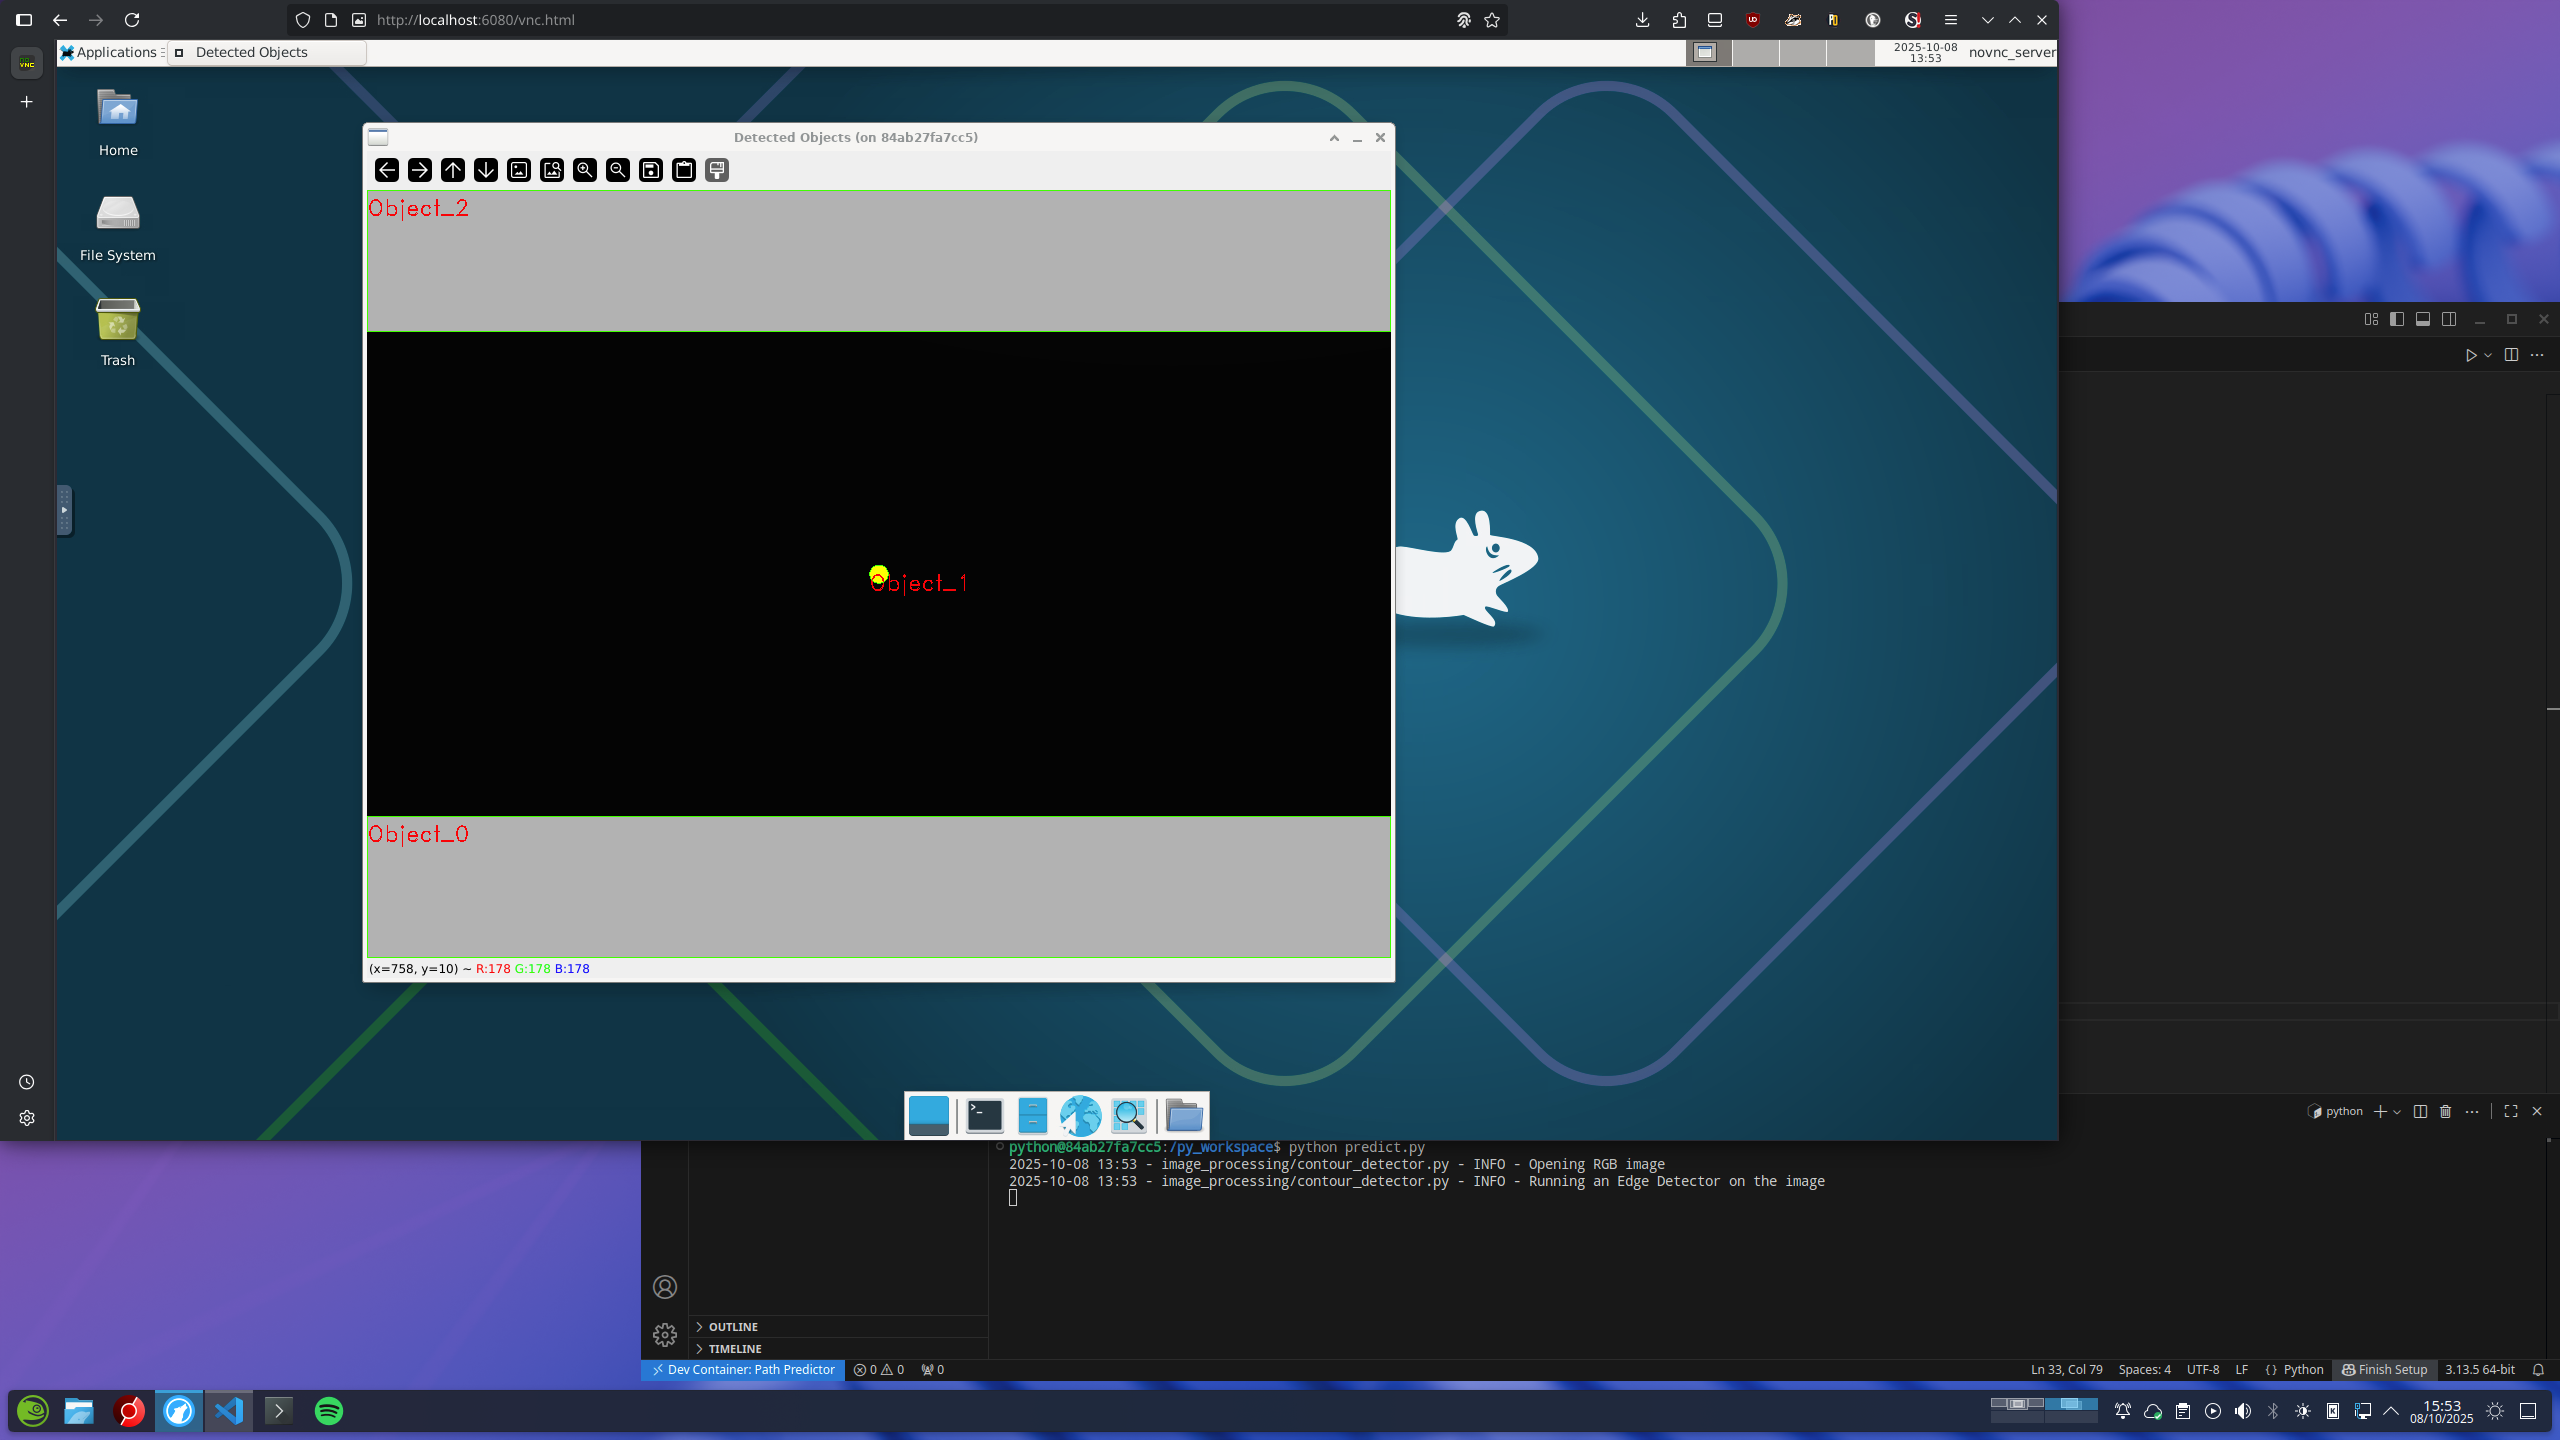
\includegraphics[width=\textwidth]{media/ContourDetector_Detection.png}
                    \end{subfigure}
                    \begin{subfigure}{\textwidth}
                        \centering
                        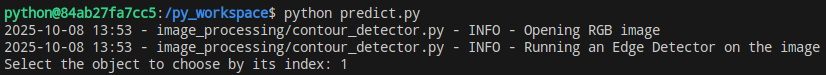
\includegraphics[width=\textwidth]{media/ContourDetector_Prompt.png}
                    \end{subfigure}
                \end{center}
            \end{figure}
        \end{column}
    \end{columns}
\end{frame}
\begin{frame}{Python Application - Pixel to World coordinates Converter}
    \begin{columns}
        \begin{column}{.35\linewidth}
            Given the simulated camera intrinsic and extrinsic parameters it computes the correspondance between the pixel coordinates and the simulated world 3D coordinates, using both the contour's pixels coordinates and the depth data coming from the PointCloud published by the depth camera itself.
        \end{column}
        \begin{column}{.65\linewidth}
            \inputminted[
                fontsize=\tiny,
                breaklines,
                firstline=234,
                lastline=237
            ]{python}{../path-predictor_workspace/image_processing/pixel_to_world.py}
            \inputminted[
                fontsize=\tiny,
                breaklines,
                firstline=239,
                lastline=242
            ]{python}{../path-predictor_workspace/image_processing/pixel_to_world.py}
            \inputminted[
                fontsize=\tiny,
                breaklines,
                firstline=245,
                lastline=258
            ]{python}{../path-predictor_workspace/image_processing/pixel_to_world.py}
        \end{column}
    \end{columns}
\end{frame}
\begin{frame}{Python Application - Duplicate Remover}
    \begin{columns}
        \begin{column}{.50\linewidth}
            Since there's the possibility that different pixels map to the same coordinates after the rounding to millimetric precision, the consecutive duplicates are dropped from the final object contour coordinates file.
        \end{column}
        \begin{column}{.50\linewidth}
            \inputminted[
                fontsize=\tiny,
                breaklines,
                firstline=55,
                lastline=65
            ]{python}{../path-predictor_workspace/image_processing/duplicate_remover.py}
        \end{column}
    \end{columns}
\end{frame}